\clearpage
\section{Testing}
\label{sec:testing}

This is the test result that conducted with \ac{ATDD} method, assisted with testing framework of Velocity\index{Velocity} with others such as Cucumber\index{Cucumber}, Mocha\index{Mocha}, Chai\index{Chai}, or Jasmine\index{Jasmine}.
Actually the tests are performed in the beginning and end of software code development.
The tests are combined from unit testing, integration testing, and end-to-end testing; regarding the feature requirements to test.

In the beginning or even in the middle of the development like when doing refactoring, the feature files with Gherkin syntax are created, if those tests are conducted with Cucumber.
It can be created one by one, or even numerous of them at the same time.
One snippet of them is like in listing \autoref{lst:satellid-gherkin}.

\begin{listing}[!htb]
  \caption{Snippet of feature file for Satellid in Gherkin}
  \inputminted{ruby}{\dir/include/code/.snippets/satellid-gherkin.txt}
  \label{lst:satellid-gherkin}
\end{listing}

And then the executable file, or the actual code that can be written in JavaScript or CoffeeScript, is written like in listing \autoref{lst:satellid-gherkin-exe}.

\begin{listing}[ht]
  \caption{Executable feature file for Satellid}
  \inputminted{javascript}{\dir/include/code/.snippets/satellid-gherkin.js}
  \label{lst:satellid-gherkin-exe}
\end{listing}

Once all of the code that specified and tested are passed, it shows the green status like in \autoref{fig:satellid-app-test} in the browser that accessed within development phase.
If there

\begin{figure}[htb]
  \centering
  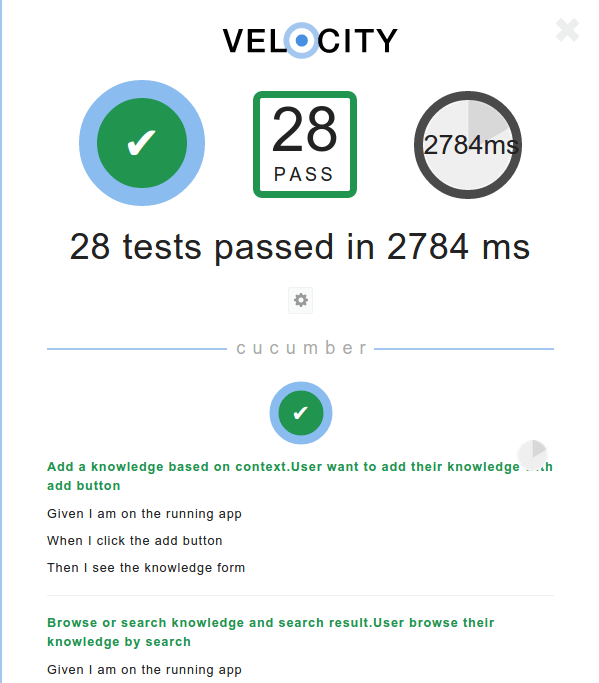
\includegraphics[height=10cm]{\dir/include/satellid-app-test.png}
  \caption{Piece of screenshot of passed Velocity test}
  \label{fig:satellid-app-test}
\end{figure}
